\chapter{Task}

I task rappresentano le azioni da eseguite concorrentemente nel sistema. 

\begin{itemize}
	\item Dal punto di vista del progettista:
	\begin{itemize}
		\item sono dei moduli software che impegnano il microprocessore per un certo periodo;
		\item permettono di eseguire calcoli e/o azioni di I/O;
		\item possono essere sostituiti, alterati o modificati in base alle necessità.
	\end{itemize}
	\item Dal punto di vista dell'utente invece:
	\begin{itemize}
		\item  creano l'illusione di avere un unico sistema monolitico;
		\item  la semplice esistenza e quindi la loro gestione è trasparente all'utente.
	\end{itemize}
\end{itemize}

\newpage
\subsection{Generalizzazione del funzionamento di un task}
\begin{figure}[!ht]
	\centering
	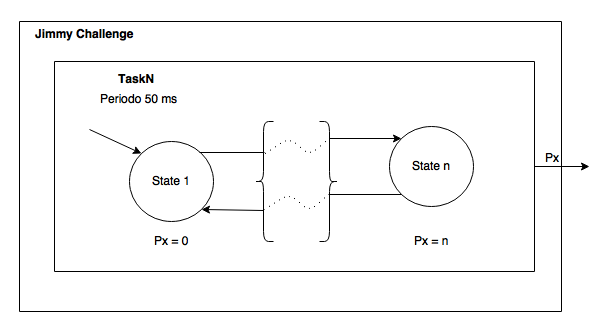
\includegraphics[scale=.60]{img/task_generic.png}
	\caption{Generalizzazione dei task}
\end{figure}

\subsubsection{Elenco dei Task sviluppati:}
\begin{enumerate}
	\item SonarTask
	\item ButtonTask
	\item BuzzerTask
	\item LedTask
	\item LedPwmTask
	\item LedRgbTask
\end{enumerate}

\section{Le espressioni Lambda in Wiring/C++11}

Una \textbf{Lambda expression} (\textit{lambda closure}) è una funzione anonima definita al momento della chiamata. 

Sintassi accettate dal compilatore di Arduino:
	\begin{lstlisting}[language=C++]
		[ capture-list ] ( params ) { body }
		[ capture-list ] { body } 
	\end{lstlisting}
Caratteristiche:
\begin{itemize}
	\item La capture list è la lista di variabili che è possibile utilizzare oltre agli argomenti della funzione.
\begin{itemize}
	\item Se si definisce [\&], tutte le variabili locali saranno passate per riferimento.
	\item Se non viene specificato niente, la lambda function non ha variabili come argomenti e viene indicata con [];
\end{itemize}
	\item Il tipo di ritorno è void, a meno che non viene specificato diversamente;
	\item Il body della funzione che si trova tra parentesi graffe rappresenta le azioni che devono essere eseguite.
\end{itemize}

Vantaggi:
\begin{itemize}
	\item Completamente dichiarativa.
	\item codice chiaro e semplice da leggere e mantenere
\end{itemize}



